\chapter{Theoretical Foundations and Methodology}
\label{chap:methodology}

\section{Formal Model of Swarm Networks}
\label{sec:formal_model}

A swarm network is represented as a dynamic graph $G(V,E,t)$ evolving over time. The set of vertices corresponds to swarm agents:
\begin{equation}
V = \{v_1, v_2, \ldots, v_n\},
\label{eq:vertices}
\end{equation}
where $n$ denotes the swarm size, which may change as nodes join or leave the system.

The set of edges $E(t) \subseteq V \times V$ models communication links at time $t$: an edge $(v_i, v_j) \in E(t)$ exists when agents are within wireless range and can exchange messages. The dynamic nature of the graph reflects robot mobility, environmental obstacles, and node failures.

Each vertex $v_i$ is characterized by a state $s_i(t)$ comprising:
\begin{itemize}
  \item position $p_i(t) \in \mathbb{R}^3$;
  \item velocity $\dot{p}_i(t)$;
  \item energy level $e_i(t) \in [0, E_{\max}]$;
  \item computational resources, including processor clock frequency $f_i$ and memory capacity $m_i$;
  \item cryptographic parameters, including the current encryption key $k_i(t)$ and key length $l_i(t)$.
\end{itemize}

The global swarm state
\begin{equation}
S(t) = \{s_1(t), s_2(t), \ldots, s_n(t)\},
\label{eq:global_state}
\end{equation}
aggregates the individual node states.

Communication channels are modeled as random variables reflecting wireless conditions. The bandwidth of channel $(v_i, v_j)$ depends on inter-node distance $d_{ij}(t) = \|p_i(t) - p_j(t)\|$ and environmental noise. Channel latency $\tau_{ij}(t)$ includes propagation delay
\begin{equation}
\tau_{\text{prop}} = \frac{d_{ij}}{c},
\label{eq:prop_delay}
\end{equation}
where $c$ is the speed of light, plus processing delay $\tau_{\text{proc}}$. Packet losses $L_{ij}(t)$ model congestion, interference, or malicious jamming.

Resource constraints formalize the embedded setting: processing power is limited, memory is bounded, and depletion of $e_i(t)$ renders a node inoperable. Transmission energy consumption is proportional to the square of distance, $E_{\text{tx}} \propto d_{ij}^2$, while cryptographic operations consume energy proportional to algorithmic complexity:
\begin{equation}
E_{\text{crypto}} = \alpha \cdot C_{\text{ops}},
\label{eq:crypto_energy}
\end{equation}
where $C_{\text{ops}}$ denotes the number of cryptographic operations and $\alpha$ is the energy cost per operation.

The model supports performance analysis through throughput, end-to-end latency, and energy efficiency. Cryptographic overhead is measured by additional latency $\Delta \tau_{\text{crypto}}$ and energy consumption $\Delta E_{\text{crypto}}$ relative to unsecured transmission. The adaptive framework seeks to minimize these costs while maintaining the required security level.

A cost function $J(S(t), P(t))$ evaluates the trade-off between performance and security, where $P(t)$ denotes the vector of cryptographic parameters for all nodes. The optimization problem is defined as
\[
\min_{P(t)} J(S(t), P(t))
\]
subject to energy and latency constraints $e_i(t) > E_{\min}$ and $\tau_{ij}(t) < \tau_{\max}$. The solution determines the optimal encryption parameters for the current swarm state.
In the later benchmark prototype, this optimization view is approximated by a threshold-based selector rather than solved directly.

\section{Threat Model and Security Requirements}
\label{sec:threat_model}

The adversarial model classifies the capabilities of an attacker. A \emph{passive adversary} eavesdrops on communications, an \emph{active adversary} modifies or injects messages, and a \emph{compromised node} scenario assumes access to keys and memory. The Dolev--Yao model assumes network control with perfect cryptographic primitives; extended models account for computationally bounded adversaries and implementation-level weaknesses.

Attack types relevant to swarms include eavesdropping, message tampering, impersonation, replay, Sybil, wormhole, and denial-of-service attacks.

Confidentiality requirements protect message contents from unauthorized access. In the present thesis, confidentiality at the data-plane level is operationalized through AEAD schemes with unique nonces per encryption. This is a design requirement for the prototype rather than a claim derived from the swarm-robotics literature itself.

Authentication requirements ensure sender authenticity and message integrity. EUF-CMA (Existential Unforgeability under Chosen-Message Attack) guarantees that an adversary cannot forge a valid signature for a new message after observing chosen-message queries. Digital signature schemes such as ECDSA and Schnorr provide EUF-CMA under standard cryptographic assumptions, while MACs such as HMAC and Poly1305 provide symmetric-key authentication~\cite{nistFips198HMAC,rfc8439}.

Data integrity prevents undetected message modification. Cryptographic hash functions such as SHA-256 and Blake2 produce fixed-length digests; authenticated encryption schemes such as AES-GCM and ChaCha20-Poly1305 combine confidentiality and integrity in one step~\cite{nistSP80038DGCM,rfc8439}.

Additional security properties can strengthen swarm systems beyond the current prototype, especially resilience to node compromise and stronger protection of past sessions through rekeying. Swarm missions differ in criticality, but the prototype evaluated later in the thesis focuses on a narrower question: how switching between stronger and lighter communication profiles affects performance and model-based efficiency under constrained execution. In this thesis, confidentiality, authentication, integrity, and compromise containment are treated as the core security requirements for the executable benchmark, as summarized in Table~\ref{tab:security_requirements}.

\renewcommand{\arraystretch}{1.1}
\begin{longtable}{|>{\raggedright\arraybackslash}p{0.27\textwidth}|>{\raggedright\arraybackslash}p{0.23\textwidth}|>{\raggedright\arraybackslash}p{0.22\textwidth}|>{\raggedright\arraybackslash}p{0.16\textwidth}|}
\caption{Security Requirements and Corresponding Cryptographic Mechanisms}
\label{tab:security_requirements} \\
\hline
\textbf{Security Requirement} & \textbf{Definition} & \textbf{Mechanism} & \textbf{Swarm Application} \\
\hline
\endfirsthead
\caption[]{Security Requirements and Corresponding Cryptographic Mechanisms (continued)} \\
\hline
\textbf{Security Requirement} & \textbf{Definition} & \textbf{Mechanism} & \textbf{Swarm Application} \\
\hline
\endhead
Confidentiality (IND-CPA) &
Ciphertext is indistinguishable from random data &
AES-GCM, ChaCha20, ECC-based encryption &
Protection of sensor data and coordinates \\
\hline
Authentication (EUF-CMA-style goal) &
Runtime authenticators cannot be forged without the relevant secret &
HMAC, token-based hash chains, digital signatures for control messages &
Verification of packet origin and trusted updates \\
\hline
Data integrity &
Unauthorized modifications are detected &
Hash functions, MACs, authenticated encryption &
Prevention of message tampering \\
\hline
Compromise containment &
Rekeying limits the impact of disclosed session state &
Per-epoch ECDH and periodic key refresh &
Damage reduction after local compromise \\
\hline
\end{longtable}

\section{Mathematical Toolkit}
\label{sec:math_toolkit}

Computational complexity theory classifies algorithms according to asymptotic resource requirements. Time complexity $T(n)$ denotes the number of elementary operations as a function of input size $n$, and space complexity $S(n)$ denotes memory usage. Common classes include:
\begin{itemize}
  \item $O(1)$ --- constant;
  \item $O(\log n)$ --- logarithmic;
  \item $O(n)$ --- linear;
  \item $O(n \log n)$ --- linearithmic;
  \item $O(n^2)$ --- quadratic.
\end{itemize}
Cryptographic operations have characteristic cost patterns:
\begin{itemize}
  \item symmetric block encryption --- $O(1)$ for a fixed block size;
  \item hashing a message of length $n$ --- $O(n)$;
  \item elliptic-curve scalar multiplication --- substantially more expensive than a single symmetric-message operation on constrained platforms;
  \item modular exponentiation --- typically heavier than lightweight symmetric protection in the same environment.
\end{itemize}
For swarm systems, swarm size $n$ is critical; protocols with quadratic communication or synchronization cost become progressively less attractive as the number of participating nodes grows.

Game-theoretic models analyze interactions between legitimate agents and an adversary. In a simple security game, the defender selects a cryptographic parameter $p \in P$, the adversary selects an attack $a \in A$, and the payoff $U(p,a)$ is the attack success probability.
In a Stackelberg game, the defender commits to parameters first and the adversary responds, so the adaptation function $F$ selects parameters that increase the cost of a successful attack.

Information-theoretic security analysis evaluates fundamental limits of information protection. Shannon entropy is defined as
\begin{equation}
H(X) = - \sum_x p(x)\log p(x).
\label{eq:shannon_entropy}
\end{equation}
It measures the uncertainty of a random variable $X$. Perfect secrecy is defined by $H(M \mid C) = H(M)$, meaning ciphertext $C$ conveys no information about message $M$. Practical schemes target computational security; mutual information
\[
I(M;C) = H(M) - H(M \mid C)
\]
quantifies information leakage, and minimizing $I(M;C)$ is a protocol design objective. Secure channel capacity is expressed as
\begin{equation}
C_s = C - \varepsilon,
\label{eq:secure_capacity}
\end{equation}
where $C$ is channel capacity and $\varepsilon$ denotes leakage to the adversary.

Asymptotic performance analysis characterizes protocol scalability. Communication complexity is the number of bits transmitted between nodes. For key exchange, ECDH requires one round and communication cost proportional to the exchanged public-key material. For authentication of many messages, aggregation can reduce repeated verification overhead, although the executable benchmark in this thesis does not implement batched verification.
\begin{itemize}
  \item an $O(n)$ protocol scales linearly with swarm size;
  \item an $O(n^2)$ protocol imposes pairwise cost growth that can quickly dominate runtime and synchronization overhead.
\end{itemize}
The broader adaptive framework therefore aims to avoid unnecessary pairwise coordination work, even though the benchmarked prototype later in the thesis is intentionally restricted to a pairwise data path.

Probabilistic analysis models random failures and attacks. Let the probability of node compromise be $p_c$; then the number of compromised nodes follows
\[
N_c \sim \mathrm{Binomial}(n, p_c).
\]
Under threshold cryptography, a secret is reconstructible from $t$ out of $n$ nodes; the probability of secret loss is
\begin{equation}
P_{\text{fail}} = \sum_{k=t}^{n} \binom{n}{k} p_c^k (1-p_c)^{n-k}.
\label{eq:threshold_failure}
\end{equation}
Choosing $t$ is a security-availability trade-off. Message delay can be modeled by an exponential distribution $\tau \sim \mathrm{Exp}(\lambda)$, yielding
\[
P(\tau > \tau_{\max}) = e^{-\lambda \tau_{\max}}.
\]
Shorter keys reduce $\tau$ but increase $P_{\text{break}}$, whereas longer keys improve security at the cost of higher delay.

Optimization methods cast protocol design as a mathematical programming problem. A typical objective minimizes a weighted sum of delay, energy, and risk:
\begin{equation}
J = w_1 \tau + w_2 E + w_3 R,
\label{eq:objective}
\end{equation}
where $w_i$ are weighting coefficients. Constraints include node energy $e_i > E_{\min}$, latency $\tau < \tau_{\max}$, and security risk $R < R_{\max}$. Decision variables include key length $l$, rotation frequency $f_{\mathrm{rot}}$, the data-plane cipher $a \in \{\mathrm{AES}, \mathrm{ChaCha}\}$, and the runtime authentication mode $m_{\mathrm{auth}}$. In the benchmarked prototype, $m_{\mathrm{auth}}$ is either HMAC-SHA256 or a sequence-bound hash token. If $J$ is convex, the optimum can be found efficiently; otherwise, heuristic methods may be required.

This toolkit provides the basis for the performance bounds and security proofs derived later (Fig.~\ref{fig:math_foundations}).

\begin{figure}[H]
\centering
% Export the Mermaid diagram (SVG/PDF/PNG) and place it in figs/ if you want LaTeX compilation.
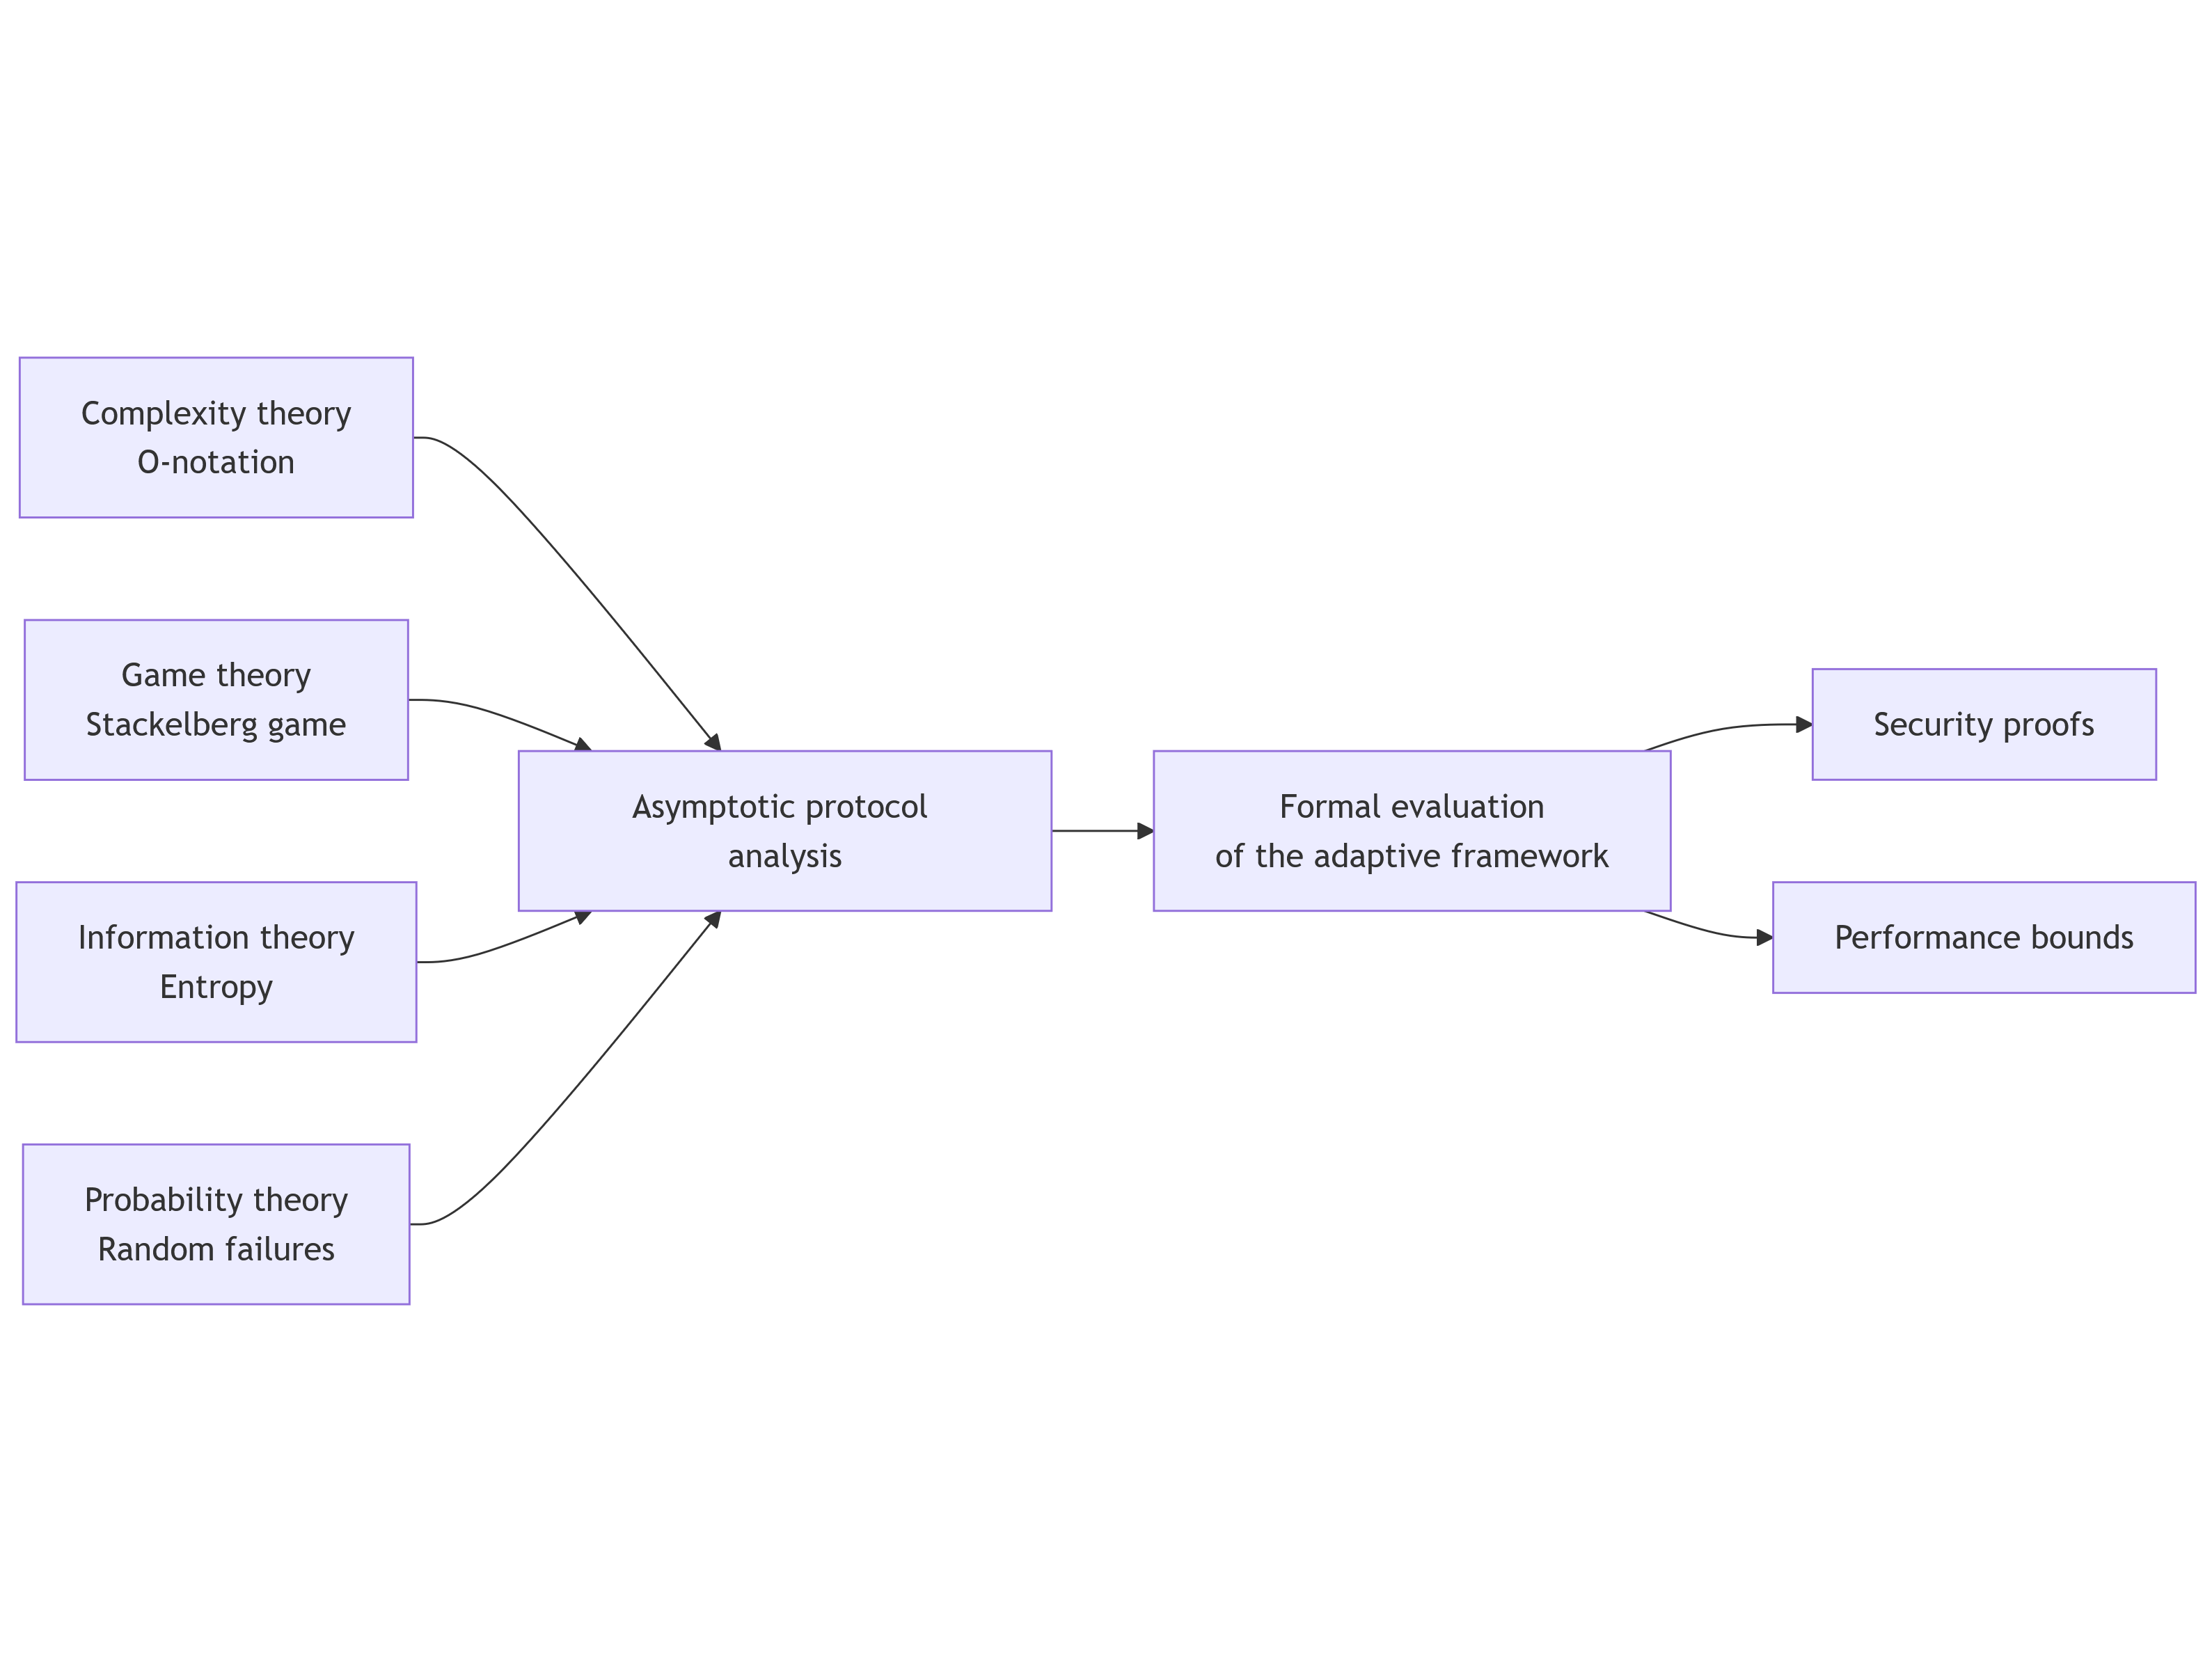
\includegraphics[width=\textwidth]{figs/math_foundations.png}
\caption{Mathematical foundations for analyzing the adaptive framework.}
\label{fig:math_foundations}
\end{figure}

The diagram visualizes the integration of theoretical disciplines used later in the thesis.


\section{Methodology Overview}
\label{sec:methodology_overview}

The research methodology is structured into sequential stages. \textbf{Stage 1: literature consolidation} reviews ECC-based key exchange, symmetric encryption with pre-shared keys, and token-based authentication, then summarizes their complexity, overhead, and security trade-offs~\cite{adeniyiSystematicReviewECC2024,kumarComprehensiveSurveyAuthenticationIoT2022}.

\textbf{Stage 2: theoretical framework development} defines the swarm graph, the threat model, the security requirements, and the adaptation function $F$, together with the optimization objective $J(S,P)$.

\textbf{Stage 3: complexity analysis of baseline protocols} derives relative computational bounds for each protocol. For ECC--ECDH, scalar multiplication is treated as the dominant setup cost, while communication cost is proportional to the exchanged public-key material. For AES-GCM:
\begin{itemize}
  \item block encryption is $O(1)$ per block;
  \item authentication is $O(n)$ for a message consisting of $n$ blocks.
\end{itemize}
For hash-chain tokens, generation of a chain of length $L$ costs $O(L \cdot h)$ and token verification costs $O(h)$. Communication overhead is summarized through message sizes, and protocols linear in the number of nodes are preferred for large swarms.

\textbf{Stage 4: retained formal security analysis} identifies vulnerabilities and attack vectors, then connects the data-plane confidentiality and authentication goals to standard assumptions about the employed primitives. The purpose of this stage is to bound the claims made later in the thesis, not to present a full end-to-end proof of the adaptive benchmark implementation.

\textbf{Stage 5: adaptive framework design} develops the adaptation function $F: S(t) \rightarrow P(t)$. At the architectural level, network density is expressed as
\begin{equation}
\rho = \frac{n}{A},
\label{eq:density}
\end{equation}
where $A$ is the coverage area. The average energy level is
\begin{equation}
\bar{e} = \frac{1}{n}\sum e_i.
\label{eq:avg_energy}
\end{equation}
Threat level $\theta \in [0,1]$ is estimated from anomaly detection. Tuning parameters include key length $l \in \{192,256\}$ for the AES-based profiles used in the benchmark, a ChaCha20-Poly1305 lightweight profile, a scenario-fixed rekey interval, and the runtime authentication mode. The prototype uses HMAC-SHA256 for the AES-based profiles and a sequence-bound hash token for the lightweight profile. The cost function is defined as
\begin{equation}
J = \alpha \tau(l,a,m_{\mathrm{auth}}) + \beta E_{\mathrm{crypto}}(l,a,m_{\mathrm{auth}}) + \gamma R(\theta,l,m_{\mathrm{auth}}),
\label{eq:cost_function}
\end{equation}
where $\tau$ is latency, $E_{\mathrm{crypto}}$ is a platform-dependent energy term, and $R$ is a symbolic residual-risk term. In the executable prototype, the decision procedure is simplified to:
\[
\text{if } \theta \geq \theta_{\mathrm{high}} \text{ then select heavy profile;}
\]
\[
\text{else if } \bar{e} \leq E_{\mathrm{crit}} \text{ then select lightweight profile;}
\]
\[
\text{else select balanced profile.}
\]

\textbf{Stage 6: protocol specification} describes the initialization, operational, and adaptation phases of the prototype actually evaluated later: agents establish pairwise keys with X25519-based exchange, derive symmetric material with HKDF, and switch among heavy, balanced, and lightweight data-plane profiles according to scripted threat and energy inputs.
\begin{equation}
P(t) = F(S(t)),
\label{eq:adaptation}
\end{equation}
The broader density-aware and consensus-aware design remains a conceptual extension rather than a benchmarked implementation artifact.

\textbf{Stage 7: practical benchmark evaluation} runs the implemented protocol under constrained CPU and memory budgets, compares static-heavy, static-balanced, static-lightweight, and adaptive modes, and records measured latency, throughput, switching behavior, and normalized energy proxies.

\textbf{Stage 8: design guidelines formulation} translates the findings into practical recommendations for scenario-specific parameterization, primitive selection, and secure deployment.

The methodology provides a path from formal modeling to design, implementation, and benchmark-based evaluation of an adaptive framework, while keeping the security--performance trade-off explicit.
